\section{Introduction}

The Vera C.\ Rubin Observatory is located on Cerro Pach\'{o}n in Chile and consists of the 8.4\,m Simonyi Survey Telescope and the 1.2\,m Rubin Auxiliary Telescope.
Over the course of 10 years the Rubin Observatory will take data for the Legacy Survey of Space and Time (LSST) and deliver 11 data releases \cite{2019ApJ...873..111I}.
The Rubin Observatory generates a data volume of approximately 20\,TB per night and this data is handled using a Data Management System \cite{2022arXiv221113611O} that transfers the files from the summit to the US Data Facility hosted at the SLAC National Accelerator Laboratory (SLAC), triggers the pipeline processing, and makes the data available to the data access centers.
The LSST Science Pipelines \cite{2019ASPC..523..521B} will be used to process the data and are designed such that neither the pipeline algorithmic code nor the scientist inspecting the data know where the data are stored or what data format they are stored in.
The software abstraction layer we use for this is called the Data Butler. \cite{2019ASPC..523..653J,2022SPIE12189E..11J}

\section{The Data Butler}

The Rubin Observatory Data Butler concept has been in the data management plan from the very early days of the project \cite{2007ASPC..376....3K,2010SPIE.7740E..15A}.
In 2017 \cite{LDM-563} we decided to rewrite the Butler library from scratch to take into account new technologies, clarified requirements, \cite{LDM-556} and lessons learned from previous implementations.
This version, colloquially known as the ``generation 3 middleware'', was formally accepted by the project in 2022. \cite{DMTR-271}

The Data Butler has been described in a previous paper \cite{2022SPIE12189E..11J} and a simple block diagram is shown in Fig.~\ref{fig:direct}, but the important concepts of dimension records, data coordinates, collections, dataset types, and formatters are summarized here.

\begin{figure}
\centering
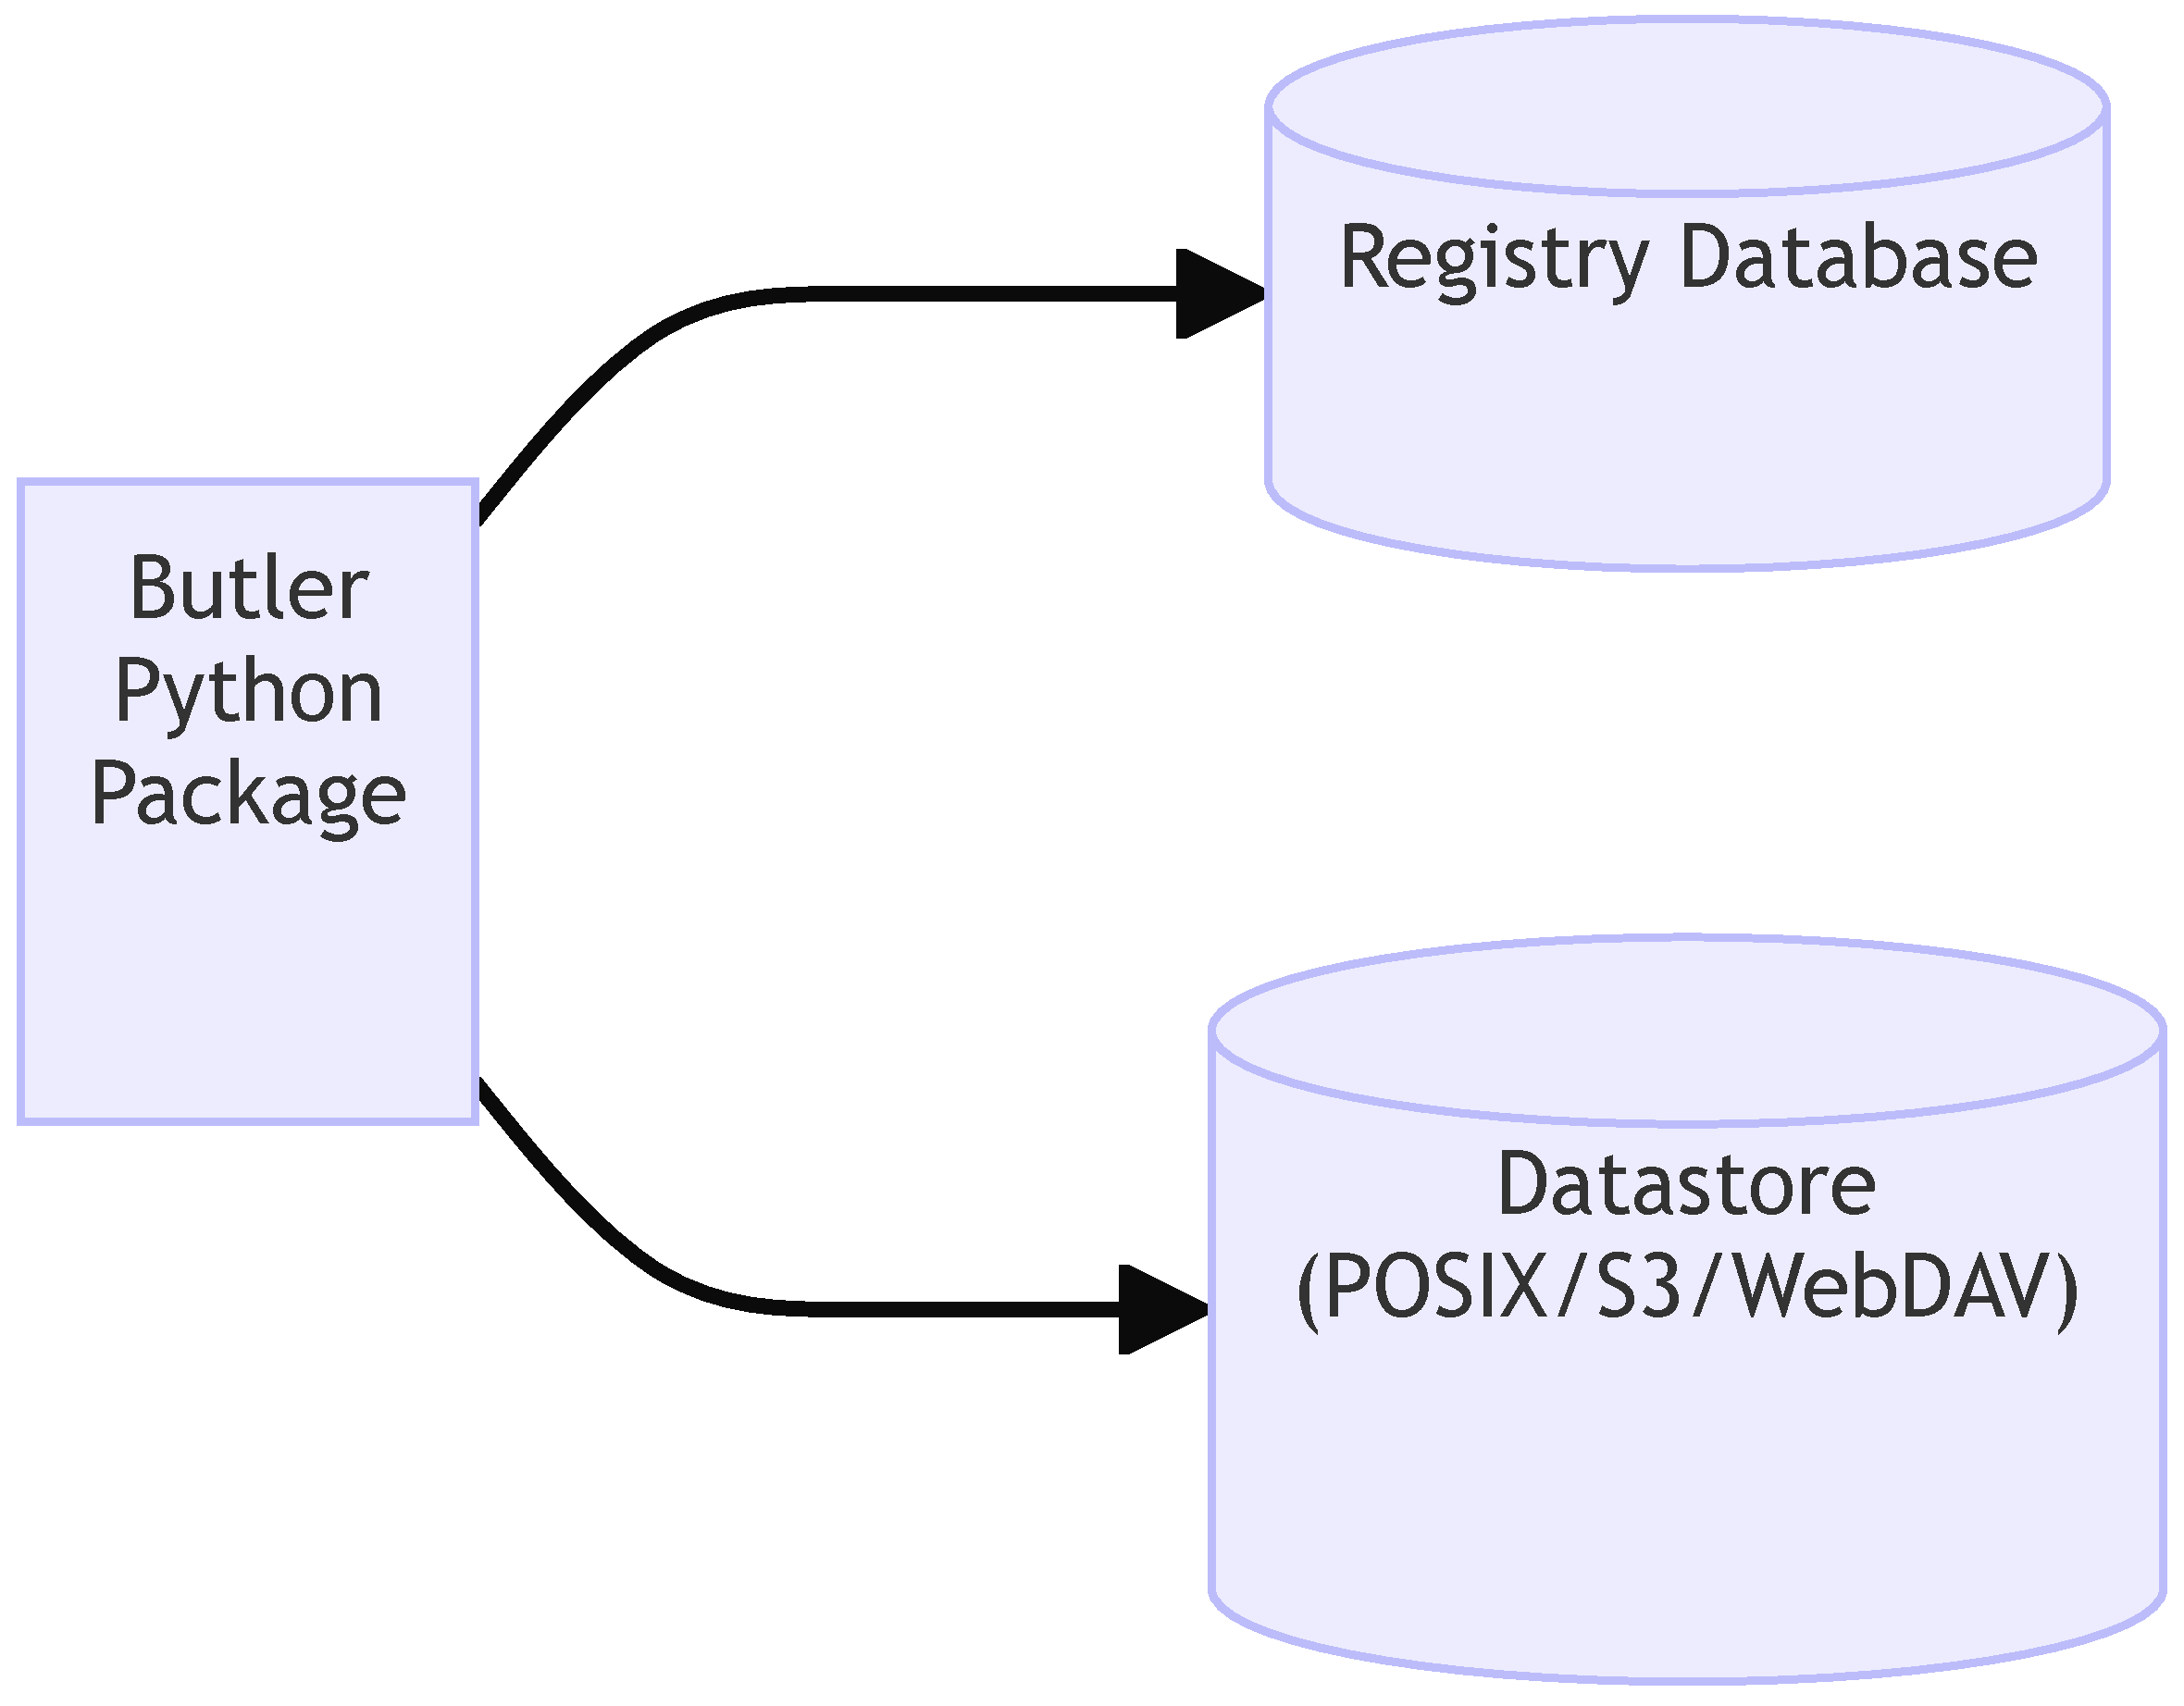
\includegraphics[width=0.5\textwidth]{butler-direct}
\caption{The direct butler architecture. A client connects directly to a database and a datastore. The datastore can be a POSIX file system, WebDAV server, or an S3 object store. The database registry can either be SQLite for testing or PostgreSQL.\label{fig:direct}}
\end{figure}


\subsection{Dimension Records and Coordinates}

The Butler registry assigns datasets specific coordinates within a dimensional space (what we call a ``dimension universe'').
These dimensions generally refer to scientifically useful concepts such as the instrument, an observation on the sky, or a patch on the sky.
Some common examples of dimensions used at the Rubin Observatory are listed in Table\,\ref{tab:dimensions}.
These dimensions and associated coordinates (which can only be strings or integers) are created when new observations are ingested or when new instruments or skymaps are defined.

\begin{table}[ht]
\caption{Common dimensions present in the default dimension universe.}
\centering
\begin{tabular}{|l|l|}
\hline
\texttt{instrument} &  The instrument that generated this data. \\ \hline
\texttt{band} & Waveband of interest.  \\ \hline
\texttt{detector} & A specific detector within the instrument. \\ \hline
\texttt{physical\_filter} &  Filter used for the exposure. \\ \hline
\texttt{day\_obs} & The observing day. \\ \hline
\texttt{group} &  Grouping identifier. \\ \hline
\texttt{exposure} & Individual exposure. \\ \hline
\texttt{visit} &  Up to 2 exposures taken sequentially at the same sky position. \\ \hline
\texttt{tract} &  Tesselation of the sky. \\ \hline
\texttt{patch} &  Patch within a tract.\\ \hline
\end{tabular}
\label{tab:dimensions}
\end{table}

\subsection{Dataset Types}

A ``dataset type'' describes an input or an output from a data processing task in a general way.
The name of the dataset type is meaningful to the pipeline user or scientist with examples such as ``raw'' (a file that comes straight from the instrument), ``calexp'' (a calibrated single exposure), or ``coadd'' (a generic stack of multiple images).
The dataset type also specifies the relevant dimensions -- a ``raw'' might be described by \texttt{exposure}, \texttt{instrument}, \texttt{detector} but an output co-add might be described by \texttt{tract}, \texttt{patch}, \texttt{skymap}, and \texttt{band}.

The final part of a dataset type is the ``storage class''.
The storage class is a proxy for the Python type that will be used.
Along with the Python type it can also describe individual components (such as metadata or image, variance, or mask) which are declared to be retrievable independently, and also specify conversion methods to handle cases where a pipeline task returns something that is compatible with the underlying storage class but is not identical.

\subsection{Collections}

Every dataset in a Butler repository must be stored in a \texttt{RUN} collection.
This collection can be thought of as representing a folder or directory, although there is no requirement that a file will be written somewhere.
A single \texttt{RUN} collection can contain any number of datasets so long as a dataset does not already exist in that collection with an identical dataset type and data coordinate.

A \texttt{CHAINED} collection consists of a list of collections that will be searched in order.
These collections can contain more \texttt{CHAINED} collections.
A \texttt{CHAINED} collection is usually created during a data processing campaign and generally consists of all the input collections and a timestamped collection.
This allows a single output collection to be used to find all the inputs and outputs and the timestamped name allows resubmissions to be stacked using additional timestamped names.

A \texttt{TAGGED} collection is used to create a bespoke collection containing a curated list of datasets.
The only requirement is that there are no duplicate dataset type / data coordinate combinations.

A \texttt{CALIBRATION} collection is a special type of collection that does allow duplicated dataset type and data coordinate combinations but uses validity timespans to break any ambiguity.
This allows a raw exposure, which is implicitly anchored in time, to be associated with the relevant processed calibration datasets.

\subsection{Formatters}

A Butler datastore enables provides an additional abstraction layer within Butler that decouples the serialization and storage of a dataset from knowledge of its existence.
Datastores exist that can write directly to the Rubin Observatory metrics database \cite{2024SPIE13101.59Ftmp} and talk to multiple datastores as if they were one datastore, but the most commonly-used datastore implementation is one that reads and writes files.
When a file-backed datastore is given a Python object it uses a Python formatter class to serialize it to bytes and, conversely, when someone requests a dataset the datastore reads the bytes and uses the formatter to convert it to a Python object.
The choice of formatter class is controlled by datastore configuration and is selected by comparing with the storage class or dataset type.

\section{Moving to the Cloud}

The original operating plan for the LSST was to host the data at the National Center for Supercomputing Applications in Champaign-Urbana. \cite{2012SPIE.8451E..0VF}
In this scenario the 10,000 science users that the archive was sized to support would all be given accounts directly at the archive center and access would be controlled directly on the file system using ACLs and on the databases using database accounts.
With the move to SLAC as the archive center \cite{RTN-021} this approach was no longer feasible given that SLAC is a Department of Energy facility which has much tighter controls over who can be issued computer accounts and a much more detailed background check.
Ten thousand accounts would take a significant amount of time to be processed and it was unacceptable to the project that some science users with data rights might not be able to acquire accounts at all.

To solve this problem the project adopted a ``hybrid cloud'' solution \cite{2024SPIE13101.86Otmp} where all the science users will be using the Rubin Science Platform \cite{LDM-542} and be hosted on a commercial cloud where they will be given access via their educational instititution's accounts, but the data would be stored at the US Data Facility at SLAC.
In this way the DOE would not need to vet 10,000 users and we would proxy access through our infrastructure.
We prototyped cloud hosting on Google using one of our Data Previews \cite{2021arXiv211115030O} and demonstrated that the deployment, data access, and user support would work correctly with a few hundred science users.
The Data Previews, though, stored the data in the cloud and used shared authentication credentials for data access -- for LSST Data Releases the data volume will be too large to host on the cloud, with our current budget profile, and we are required to provide per-user and per-group access controls.

To support this hybrid cloud approach and to provide scalability for 10,000 users on day one of a data release, we were required to rethink our approach to the Butler and re-engineer it to use a client/server architecture.
In this way the server can use standard Rubin Science Platform authentication, \cite{DMTN-182} utilize signed URLs to access the data at the USDF without requiring SLAC accounts, \cite{DMTN-284} and allow for a backend infrastructure that can make use of cloud resources to scale with spikes in load.

\section{Migrating to a Client/Server Architecture}

\begin{figure}
\centering
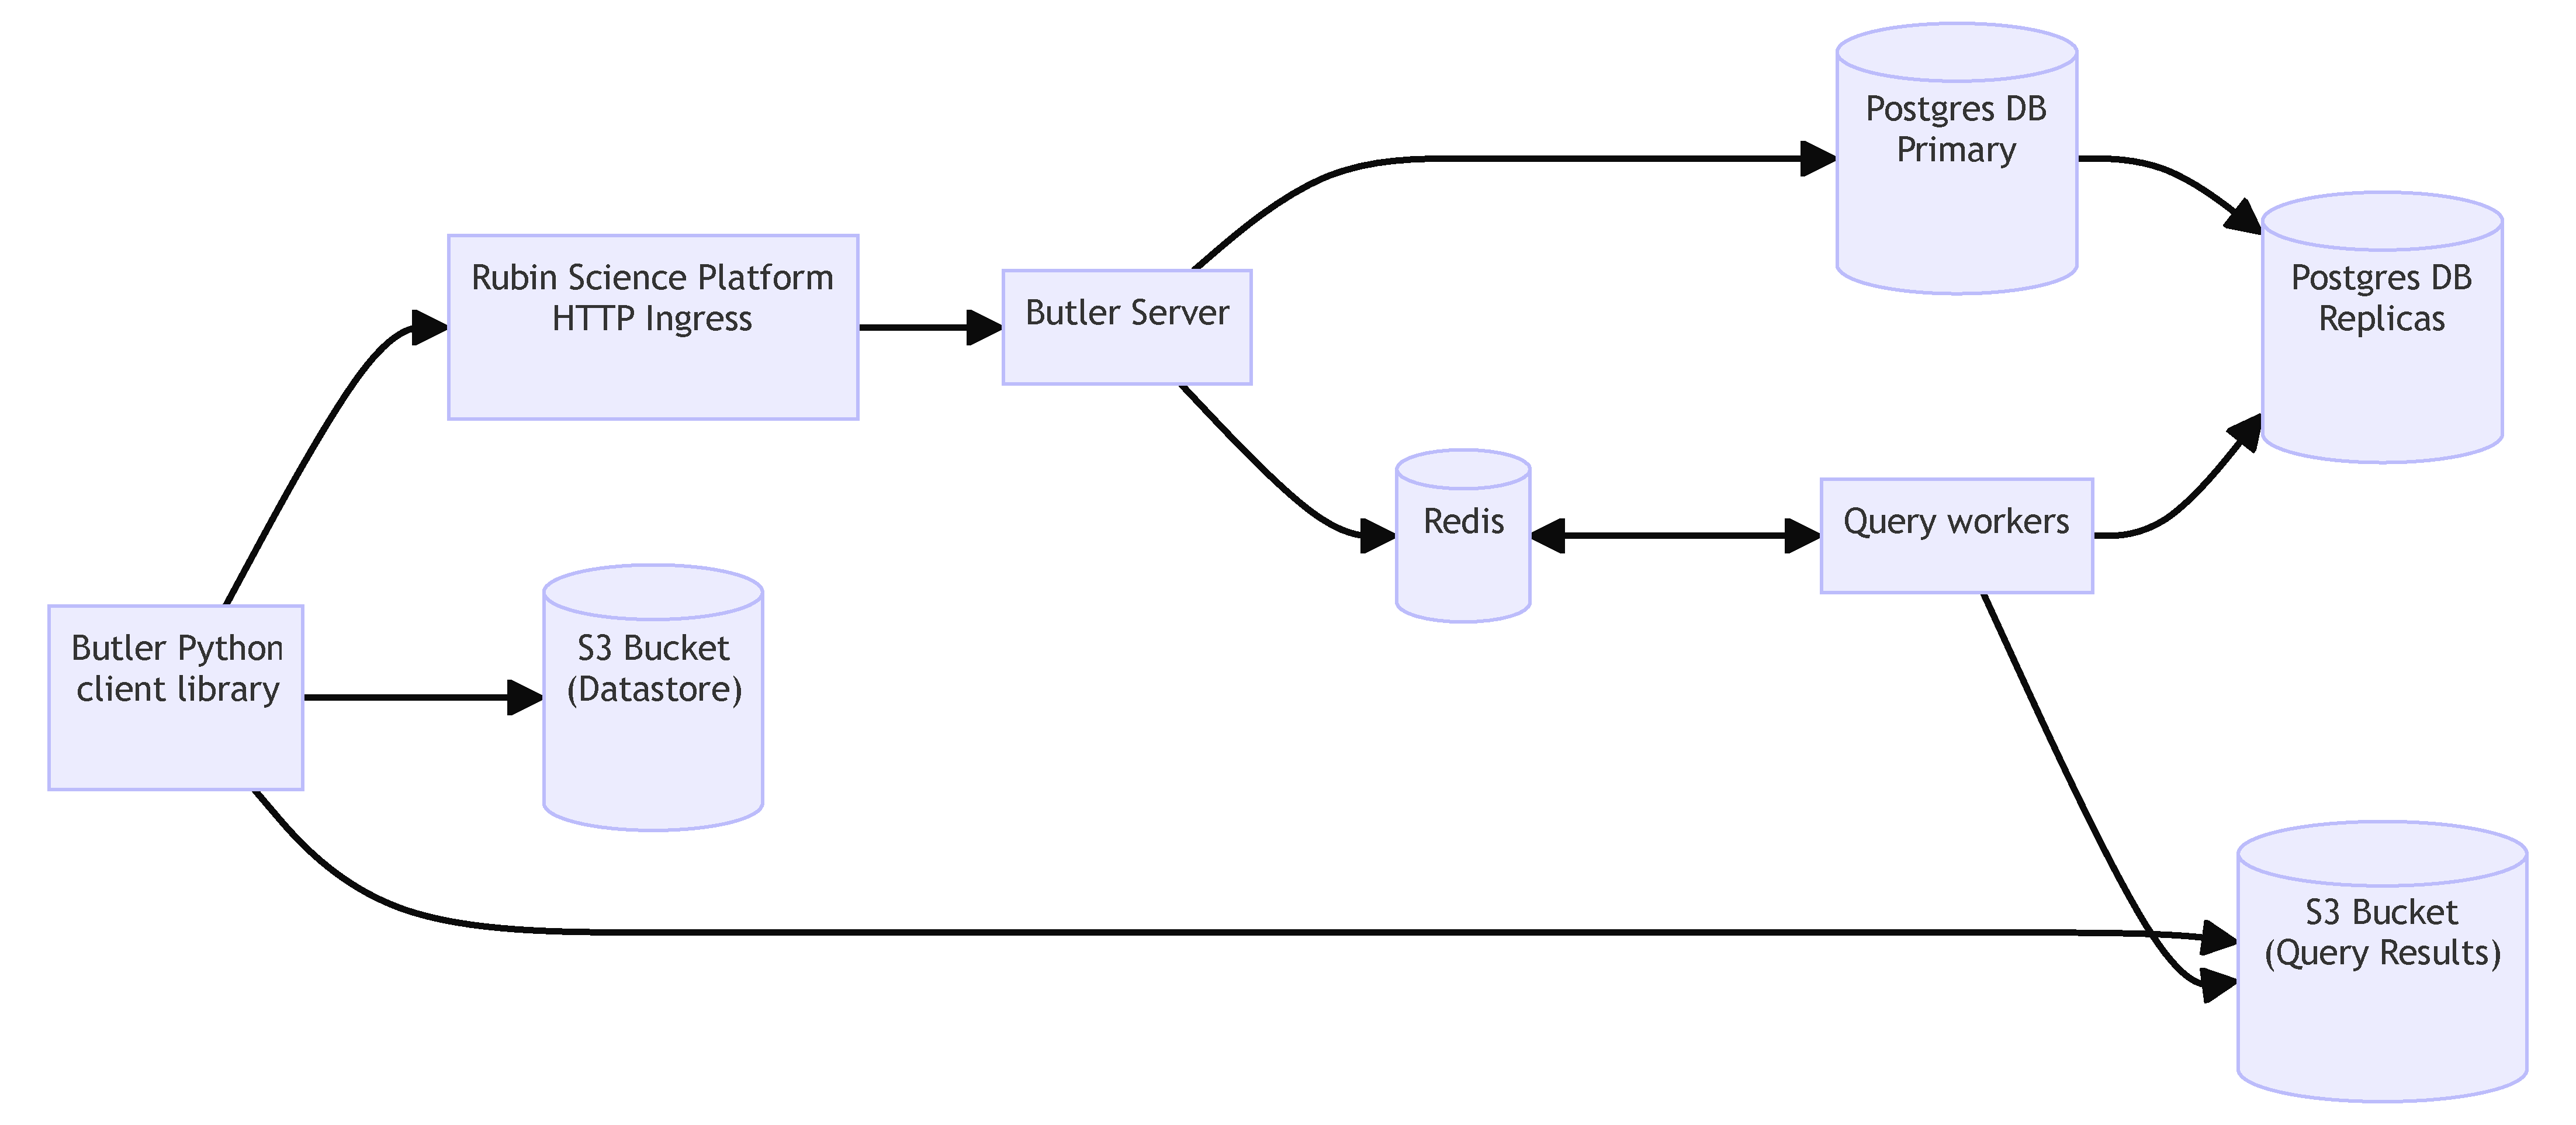
\includegraphics[width=\textwidth]{butler-client-server}
\caption{The client/server butler architecture. A client connects directly to a service which mediates the database connection and provides signed URLs to the S3 buckets.\label{fig:server}}
\end{figure}

The delivered Butler uses a direct connection to a database (generally PostgreSQL) and direct access to either a POSIX file system, an object store (supporting either Google Cloud Storage or Amazon S3), or a WebDAV server.
There is no fine-grained access control restricting database access and object store access is generally all or nothing.
For a POSIX file system datastore it is possible to restrict file system access based on ACLs.
We call this implementation the ``direct butler'' to distinguish it from the ``remote butler'' that connects to a butler server.

For Data Preview 0.2 \cite{RTN-041} this was the system we used -- anybody could read and write anything with no group or user restrictions.
For a deployment that was mainly used as a test bed and which was using previously published simulated data this was not an issue.
This approach to authentication and authorization is acceptable when running batch processing at the USDF where the campaign processing team and developers are Rubin Observatory staff, but a new approach is needed for the hybrid cloud scenario with external science users for formal data releases.

For a formal data release or access to the prompt products database, the requirements become stricter:

\begin{itemize}
\item Data products are only visible to data rights holders until the two-year proprietary period is exceeded.
\item Data rights holders can all see the formal data products but can not delete or modify them and can not write to any of the data release collections.
\item Data rights holders should be allowed to store their own derived products and no-one else should be able to access them or even know they exist.
\item Data rights holders should be allowed to collaborate with others and make use of shared collections that are private to their group.
\item File quotas will be used to ensure fairness, although a petition can be made to increase the default quota.
\end{itemize}

To satisfy these requirements the only option is to move to a web services architecture.
We refer to this implementation as the ``remote butler'' where the client sends messages to a server, the server checks the authentication tokens, decides whether the user has access to the dataset or collections, and then uses the ``direct butler'' to process the request.
The server can also sign URLs and return them to the client which is then responsible for retrieving the dataset and reading it into memory.
A block diagram with the architecture is shown in Fig.~\ref{fig:server}.

Replacing direct connections to databases and file systems with a web service does complicate some of the Butler design and we have been forced to make some fairly major internal changes.
The ``direct butler'' implementation must still work (that is how the server communicates with the registry) but certain assumptions are no longer valid.

For example, during graph-building, the process whereby we take a pipeline definition and combine it with a butler query to generate an execution workflow,\cite{2023arXiv230303313L} the direct butler makes use of temporary tables in the database.
In a stateless client/server with load balancing there is no mechanism to ensure that the client is talking to the same web service or the same database server and so long-lived temporary tables may no longer be viable without significant re-architecting.
In the following sections some of these difficulties are discussed and solutions proposed.

\subsection{Configuration}

The direct Butler supports configuration via a YAML or JSON file.
The system was designed from the beginning to allow a butler to be constructed from a single configuration file which could be augmented by the user to override any of the settings including output file formatters, file templating, addition of chained datastores, file-writing compression parameters, and even storage class definitions.
If they inadvertently modified the registry or datastore definitions in an incompatible way the worst that would happen is that they wouldn't be able to connect to the butler or they might write a file to a datastore that no-one else could read.
Furthermore, many of the configurations allowed a full Python class name to be specified, for example in the definition of a storage class, or controlling which datastore was loaded.

In a client/server environment this sort of configuration flexibility is not at all desirable for two important reasons.
Firstly, a server process should not trust anything it gets from a client that can not be vetted, and secondly, a client should not load arbitrary python code based on a message it gets from a, potentially compromised, server.

This realization is requiring us to fundamentally adjust how we treat configuration in the butler:

\begin{itemize}
\item The ability for a client to inject arbitrary configuration overrides should be reassessed and possibly be replaced by an explicit system for allowing configuration of formatters and write recipes (which are important abilities during testing and development).
\item Storage class definitions must solely be read from the client system.
  The server should never need to load a storage class and is not required to have access to the LSST Science Pipelines.
\item Storage classes must be versioned for each data release (Python types might evolve over the years even if the storage class name remains the same).
\item Formatters must now be stored in the server as a label rather than a Python class and configuration in the client must map that label to a Python class.
  A client can not import a fully-qualified Python class name coming from the server.
\item The server issues signed URLs for file upload and therefore the client can not be responsible for defining the file naming template.
\item The client should not ever see registry configuration.
\end{itemize}

\subsection{Registry Queries}

With potentially 10,000 simultaneous users running queries for datasets and dimension records, it is impossible for one server to be able to handle that load with one database.
To solve this problem there will be multiple strategies:

\begin{itemize}
\item
  Servers will pre-fetch some database dimension records and collection information. \cite{DMTN-289}
\item
  Multiple server instances will be deployed with load balancing.
\item
  Multiple database server instances will be deployed.
\item
  Servers will not run database queries directly, instead they will spawn workers that will run the queries.
\item
  The number of queries a single user can execute will be limited and a queuing system employed.
\end{itemize}


\subsubsection{Regular Expressions}\label{regular-expressions}

Some of the existing Butler APIs allow a user to specify a search using a regular expression or a glob.
Regular expressions are very useful but they are a very bad idea when the regular expression is coming from a potentially untrusted source and can even be a bad idea if a valid user is trying to do something clever and ends up with something that is very complicated.
It is easy to create a regular expression that can turn into a denial-of-service attack, we are therefore proposing that regular expressions be removed from the public APIs and that we only allow globs.

\subsubsection{Dimension Record Pre-fetching}\label{dimension-record-pre-fetching}

Dimension records are used extensively and in many cases the associated record metadata is required.
If many clients all request datasets that contain coordinates \texttt{(instrument="LSSTCam", detector=4)} the server should not query the database backend every single time to look up the definitions of those IDs.
Direct Butler does pre-fetch many common dimension records but the situation in the server is much more complicated where synchronizing a shared cache between many threads becomes the primary concern, and the client code likely doesn't need to cache anything because the definitions will always be sent over the wire from the server.

For a static data release the dimension coordinate space is pre-defined and no new records will be added.
Even for a live data repository, such as the Prompt Processing repository, certain record categories are only rarely augmented and are relatively small.

For example, the number of \texttt{instrument} records is of order 10, the number of \texttt{physical\_filter} records is of order 1,000, and the number of \texttt{detector} records is of order 1,000.
These are very common dimensions and pre-fetching them into the server is very important to reduce database load.
If a new filter is added, this event can be planned for and a mechanism can be in place to invalidate the server copy to allow it to be recreated.

The dimensions relating to how we break up the sky into tracts and patches are also something that can be considered for pre-fetch.

Even for \texttt{day\_obs} the total number of records is only about 4,000 for LSSTCam over the ten year survey (twice that if LATISS is included) with limited metadata attached to those records, and for a static data release we could consider pre-fetching those.

The situation is different for \texttt{exposure}, \texttt{visit} and \texttt{group} where there can be of order 1,000 of each of those created per night (millions of records).
Those records (including metadata fields) can not be pre-fetched into the server and must be obtained from the database every time they are needed.

\subsubsection{Collection Caching}\label{collection-caching}

In a full data release where there can be many chained collections as well as tens of thousands of user collections, it is critical that a client request for a collection definition doesn't result in multiple database queries every single time.
A user will only be allowed to see their own user collections and any group collections they are part of but the total number of collections to manage will be very large.

Caching all the collection definitions in the server might be possible, so long as the cache is shared between server threads, but the issue is knowing when to invalidate the cache.
A data release will have a large number of unchanging collection definitions combined with user and group collections that can be created or disappear at any time.
A prompt processing repository will be getting new collections on a daily basis in addition to the user and group collections.
It might be necessary for specific collections to be marked as permanent to allow the servers to know that those will not be modified, but require database queries for the dynamic collections.
The approaches to collection caching are still to be worked out and we are investigating reorganizing how collections
are stored in the database to make queries on them more efficient without the recursion currently used to support chains of datastores with chains of datastores.

It might be simpler for the client to never cache collection information if the server is caching and the client will only ever see a small subset of the total number of collections.

\subsubsection{Multiple Servers}\label{multiple-servers}

A single server, however large, can not reliably handle thousands of simultaneous requests.
This is not helped by the butler APIs being designed before \texttt{async} was considered stable, requiring the server to create threads for all incoming requests and Python not currently being a language that supports good thread performance and FastAPI being optimized for async.

To allow arbitrary scaling we will deploy multiple server instances with some form of load balancing.
We are designing the server to be stateless such that any client can talk to any server at any time without having a client pinned to a specific server.

\subsubsection{Multiple Database Servers}\label{multiple-database-servers}

Deploying multiple Butler services allows client requests to be handled at scale but that needs to be matched by database capacity.
Multiple read-only clones of a data release database can scale relatively easily.
There is a complication when clients are allowed to store data in the butler in terms of replication to replicas, and this is discussed later.

\subsubsection{Query System}\label{query-system}

Many Butler queries can take minutes or even longer, and it is not desirable to lock up resources in the server process whilst waiting for these queries to complete.
The solution is to use a system where queries are sent to workers in an execution pool.
The client will be issued a job ID and can query the server to obtain the worker status.
The client will initially use polling to determine when a query has completed and we will investigate whether UWS \cite{2016ivoa.spec.1024H} is a reasonable approach.
Once a job completes the client will receive a URI to the results in either JSON or parquet format.
These results will be written with an expiry date to allow for automatic cleanup of results that are no longer
needed.
Additionally, context managers will be supported to allow the client to send a message to the server when it no longer needs the results.
If the query resulted in many results they can be written as multiple files and multiple URIs can be returned to allow the client to paginate.

Additionally, a queue system makes it possible for individual users who are doing many queries simultaneously to be rate-limited.
The system should not look like it is down for people if a single user is submitting hundreds of queries and is ahead of everyone else in the queue.

\subsection{Reading Datasets}

The direct Butler interface supports a generic ``datastore'' abstraction layer with multiple pluggable options.
Supporting arbitrary datastore configurations allows a single butler to store datasets in file-backed datastores or datastores that use databases such as the Sasquatch system.\cite{2024SPIE13101.59Ftmp}
It is even possible for users to override datastore configurations to add their own additional datastores into the chain.
For client/server Butler this flexibility is an unwanted complication since it weakens the security model and adds unnecesary complexity.
The client/server design therefore enforces support solely for file-backed datastores where the server process issues signed URLs to allow the client to download only the datasets they have been approved to see.
The client is responsible for interpreting the formatter name specified by the server to allow it to use the correct python code for converting the file back into a python object.

\subsection{Writing to a Butler}

The biggest complication in implementing client/server Butler is handling writes.
Clients will rarely need to update dimension records (those are created by instrument registration, raw data ingest, or visit definitions, which are generally thought of as administrative tasks that can, for now, use direct butler connections, although it might be necessary for users to create their own sky map definitions) but Data Rights holders will want to read datasets, construct new datasets derived from them, and store them back in a butler.

We assume that there will be far fewer writes than there will be reads and the majority of the writes will involve multi-dataset transfers from personal workspaces or from user-batch outputs \cite{DMTN-223} rather than people writing individual datasets from Jupyter notebooks.

In the baseline plan user data will be written to a SLAC object store with the server issuing a signed URL to the client to allow the upload of the file.
Once the file has been uploaded the client will inform the server to allow the registry database to be updated.

Quotas will be needed and will likely require the butler to keep track of per-user quota usage -- if a user happens to do multiple writes in parallel across multiple butlers there is a chance that they could exceed their quota but we would run daily quota verification jobs to ensure that the butler accounting is accurate.

With multiple replicas of a read-only data release registry database server we can horizontally scale and support many user queries.
Once writes are allowed it is necessary for each replica to be notified of that modification and there will be a time where the user who wrote to the registry would not see that update if they were to immediately do a get or a query.
To simplify the replication and backup situation we are considering using read-only data release registry databases and a separate user registry database -- the user registry should be significantly smaller than the data release registry.

We have not yet decided how many user databases to create: a single user database server for all user data with replicas is one option, but it is also feasible to consider giving each user their own self-contained user registry as a namespace within a larger database server.
There is also an intermediate strategy where users are assigned specific user databases, although there is a risk that you could end up with some databases having no user activity and others having all the power users.
Regardless, multiple registries is a complication for butler where the system has been designed to be able to do joins of user collections with data release collections using the database directly and supporting two or more registry databases in a single query would lead to more work having to be done by the query worker process, using more memory, in order to do the combination from multiple registry databases.

This is particularly problematic when we come to do our user-batch processing where we build up workflow execution graphs.\cite{2022arXiv221115795G,2023arXiv230303313L}
These workflow graphs require large queries and do joins across all collections and also utilize temporary tables, and this will need to be significantly redesigned if the user collections and the data release collections are in distinct databases.

\section{Conclusions}

Converting an existing library that uses direct database and object store connections to one which uses modern web service paradigms, including supporting scalability and security, is a challenging exercise.
Whilst we realized early on that such a change was needed \cite{DMTN-169,DMTN-176} other priorities and staff resourcing issues meant that we could not really begin to look seriously at the implementation until more recently. \cite{DMTN-282,DMTN-283}

We have made significant progress in the implementation of the client/server Butler this year and it is already deployed with core functionality and used by the Rubin Science Platform Virtual Observatory services. \cite{DMTN-208}
A system will be deployed in time for Data Preview 1 in early 2025. \cite{RTN-011}
